%%%%%%%%%%%%%%%%%%%%%%%%%%%%%%%%%%%%%%%%%%%%%%%%%%%%%%%%%%%%%%%%%%%%%%%%%%%
% Juan Manuel Perez Rua
%%%%%%%%%%%%%%%%%%%%%%%%%%%%%%%%%%%%%%%%%%%%%%%%%%%%%%%%%%%%%%%%%%%%%%%%%%%

\chapter{Introduction} \label{chap:intro}

Object tracking and optical flow are two of the main components in the
computer vision toolbox, and have been focus of great research efforts, 
leading to significant progress in the last years \cite{c16}\cite{c17}. 
The object tracking problem in videos consists on estimating the 
position of a target in every frame, given an initial position. On the
other hand, the optical flow between a pair of frames consists on finding a displacement vector 
for each pixel of the first image, namely a {\it dense motion  or displacement field}. Even though for several
applications a complete (i.e. for every pixel) motion-field is needed, other applications like
human-computer interaction, object editing in video or structure-from-motion,
may only focus on an interest object and thus, only a subset of motion vectors is required. 
In such scenarios combining optical flow and object tracking in a unified 
framework appears useful and the precision of the object motion description 
could be enhanced. For instance, even with modern optical flow approaches, 
the long term dense motion estimation remains a challenge \cite{c20}\cite{c22}.  At large, object trackers provide a more robust, 
longer term motion estimation featuring a global description of an object, specially after recent works based on tracking-by-detection approaches \cite{c16}\cite{c23}\cite{c24}. 
On the other side, they lack the (sub) pixel precision of dense optical flow estimators, as well as a deeper use of contextual information for bundle motion 
vector estimation. 
Even more,  object trackers and optical flow give precious hints for other fundamental tools such as 
object segmentation in video. Nevertheless,
these two techniques were not deeply studied in the literature as a unified problem. Though optical flow has been widely used as a motion 
feature for object tracking \cite{c25}, feeding a dense motion estimator with tracking information is not being fully exploited.
This being said, we introduce  a new problem which we call object flow. Thus, for a given object of interest, 
the object flow is the set of displacement vectors for every pixel that belong to the target in a first frame, 
towards another frame of the sequence. In other words, a dense displacement  field constrained to the spatial support of the object. 
Note that by definition this induces a segmentation of the target and of the motion field.


\section{Problem definition}

We can define more precisely the object flow by starting with an image sequence, say $I_t, t:0..N-1$, and an initial 
position of the interest object in the first frame of this sequence. Let $\mathcal{R} \in \Omega$ be the region corresponding to the support of the object in the
bi-dimensional grid $\Omega$. Then, the object flow is $\mathcal{O}(x) = d_{0,t}(x), \forall x \in \mathcal{R}$.
We can define more precisely the object flow by starting with an image sequence (See Fig. \ref{diagram} for a simple diagram) and an initial 
position of the interest object in the first frame of this sequence, and letting $\mathcal{R}$ 
be the region corresponding to the support of the object in 2D, such that 
$\mathcal{R} \subset \Omega$. If $\Omega$ is the set of all the possible grid positions, 
the object flow problem consist in finding the displacement vectors $d_{0,t}(x)$ from the image $I_{0}$ to $I_{t}$, $\forall x \in \mathcal{R}$.

   \begin{figure}[bhp]
      \centering
      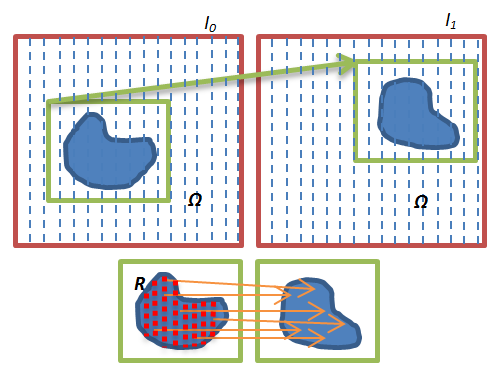
\includegraphics[width=0.66\textwidth]{../images/diagram.png}
      \caption{ Object flow definition diagram. }
      \label{diagram}
   \end{figure}

A straightforward solution to this problem would be to compute the optical flow motion field, and apply 
a segmentation mask to recover the desired motion vectors. Nevertheless, this approach carries several 
problems. For example, a globally computed optical flow method can affect small objects motion, because of 
the common use of heavy regularization priors. Moreover, even if the segmentation mask is extracted from a 
tracker window by a graph-cut based segmentation method, is likely that this mask is not going to be well suited for the 
interest object and some extra user interaction would be needed to refine this process. We propose an approach 
to reduce these problems.

\section{Objectives}

The main goal of this work is to define a dense motion descriptor for objects in video sequences. 
In order to achieve this goal, some specific objectives are defined:

\begin{itemize}

  \item To show experimentally that the idea of mixing tracking techniques with optical flow methods enhance the precision of per-object motion description.
  \item To define an automatic segmentation approach for target objects in video sequences.
  \item To establish a flow estimation method that uses the segmentation mask provided and the region of interest given by the tracker.
  \item To show experimentally that the proposed object flow method is indeed more precise than regular optical flow techniques.

\end{itemize}

\section{Document organization}

The section \ref{chap:background} starts by introducing the reader in the important topics and concepts that support the rest of this work: 
object tracking, optical flow and object segmentation. After this, in the section \ref{chap:core}, the object flow pipeline is explained in deep, 
together with the proposed algorithms. Finally, a list of results and implementation details are discussed in \ref{chap:results}.


